\chapter{Конструкторский раздел}
\label{cha:design}

В данном разделе выполняется проектирование базы данных с учетом выбранной СУБД.

\section{Диаграмма вариантов использования}

На рисунке \ref{2.1} представлена диаграмма вариантов использования (use case diagram).

\begin{figure}[ht]
  \centering
  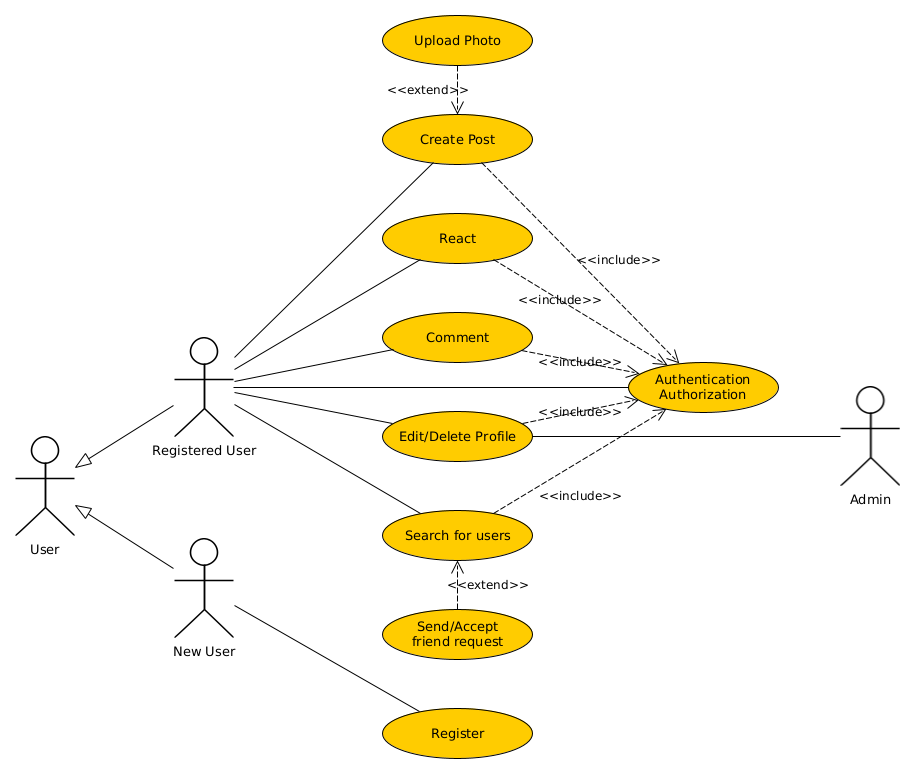
\includegraphics[width=\textwidth]{../use_case.png}
  \caption{Use case диаграмма}
  \label{2.1}
\end{figure}


\section{Диаграмма «сущность - связь»}

На рисунке \ref{2.2} представлена диаграмма сущность - связь (use case diagram).

\begin{figure}[ht]
  \centering
  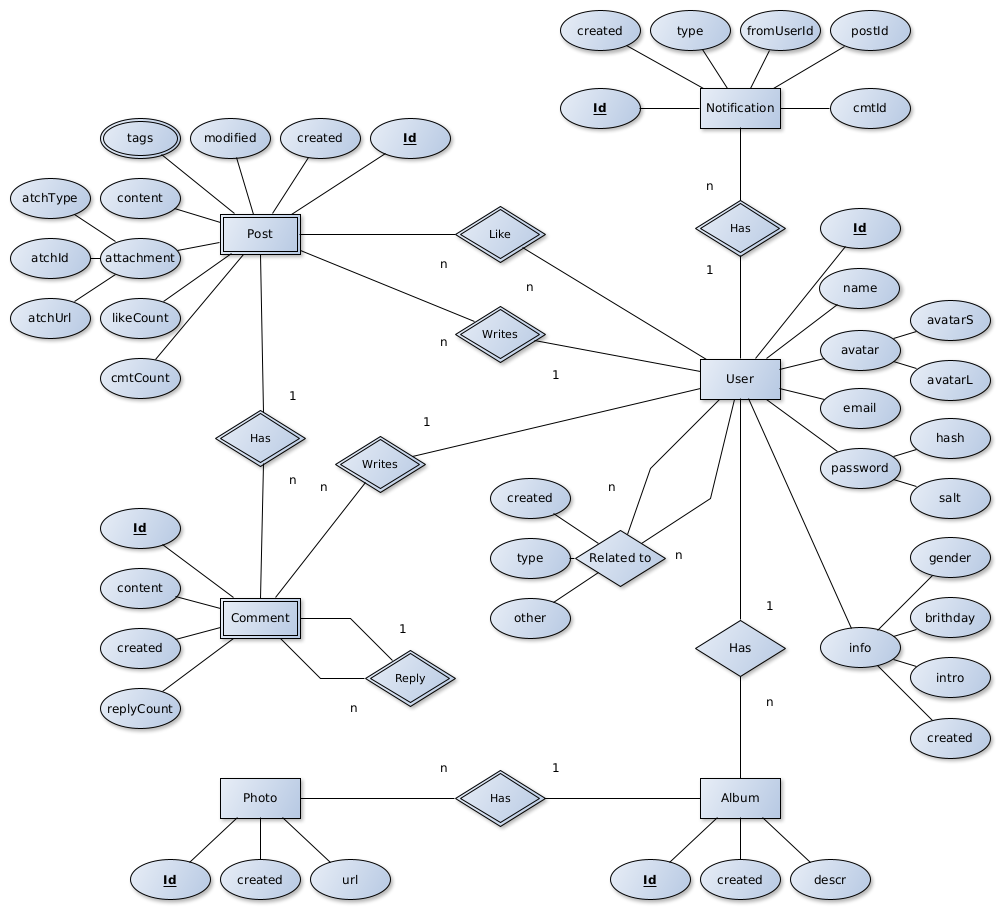
\includegraphics[width=\textwidth]{../er.png}
  \caption{ER-диаграмма}
  \label{2.2}
\end{figure}
  

\section{Проектирование таблиц базы данных}

\subsection*{Пользовательские типы данных}

\def\arraystretch{1.3}
\setlength\tabcolsep{0.5cm}

\begin{table}[H]
  \centering
  \begin{tabular}{|c|c|}
      \hline
      \bfseries Тип  & \bfseries набор значений\\
      \hline
      gender\_t & 'M','F'\\
      notif\_t  & 'like','cmt','request','accept'\\
      relation\_t & 'friend','block','request', 'follow'\\
      atch\_t & 'photo','video','poll','none'\\
      react\_t  & 'like','love','haha','wow','sad','angry'\\
      \hline
  \end{tabular}
  \caption{Пользовательские типы данных}
\end{table}

\subsection*{Таблиц базы данных}

База данных имеет 8 таблиц, показанных на рисунке \ref{2.3}.
Но ключи не показаны, но будут описаны более подробно ниже.

\begin{figure}[ht!]
  \centering
  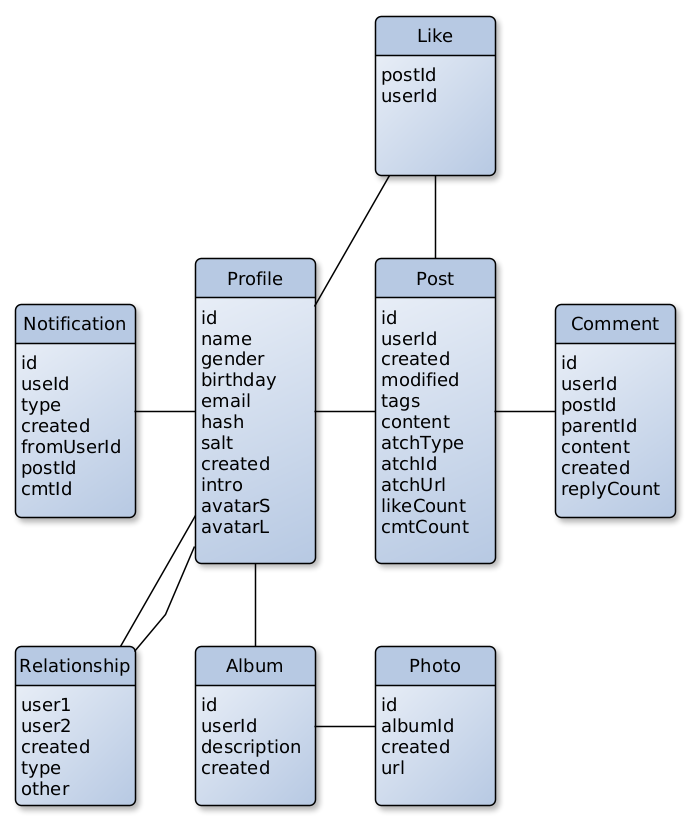
\includegraphics[width=\textwidth]{../db.png}
  \caption{Диаграмма базы данных}
  \label{2.3}
\end{figure}

% \clearpage
\def\arraystretch{1}

\begin{table}[H]
  \centering
  \begin{tabular}{|c|c|c|c|}
      \hline
      \bfseries Атрибут & \bfseries Тип & \bfseries Умолчания & Ограничения \\
      \hline
id		&	serial && 		primary key \\
name	&	varchar(32)	&&not null \\
gender	&	gender\_t &&\\
birthdate&	date &&\\
email	&	text		&&not null	unique \\
phone	&	decimal(13)	&&unique \\
salt	&	char(8)		&&not null \\
hash	&	char(28)	&&not null \\
created	&	timestamp			&default now() &\\
intro	&	text &&\\
avatarS	&	text &&\\
avatarL	&	text &&\\
postCount&	int		&default 	0 &\\
photoCount&	int		&default 	0 &\\
      \hline
  \end{tabular}
  \caption{Таблица Profile}
\end{table}


\begin{table}[H]
  \centering
  \begin{tabular}{|c|c|c|c|}
      \hline
      \bfseries Атрибут & \bfseries Тип & \bfseries Умолчания & Ограничения \\
      \hline
id		&	serial &&	primary key \\
userId	&	int		&&not null	references Profile(id)\\
created	&	timestamp			&default now() &\\
tags	&	text	&default 	'' &\\
content	&	text &&\\
atchType&	atch\_t	&default 	'none' &\\
atchId	&	int		&default 	0 &\\
atchUrl	&	text	&default 	'' &\\
reaction&	int[6]  &&\\
cmtCount&	int		&default 	0 &\\
      \hline
  \end{tabular}
  \caption{Таблица Post}
\end{table}


\begin{table}[H]
  \centering
  \begin{tabular}{|c|c|c|c|}
      \hline
      \bfseries Атрибут & \bfseries Тип & \bfseries Умолчания & Ограничения \\
      \hline
id		&	bigserial &&			primary key \\
userId	&	int		&&not null	references Profile(id)\\
postId	&	int		&&not null	references Post(id)	\\
parentId&	int &&\\
content	&	text &&\\
created	&	timestamp			&default now() &\\
      \hline
  \end{tabular}
  \caption{Таблица Comment}
\end{table}


\def\arraystretch{0.92}

\begin{table}[H]
  \centering
  \begin{tabular}{|c|c|c|c|}
      \hline
      \bfseries Атрибут & \bfseries Тип & \bfseries Умолчания & Ограничения \\
      \hline
userId 	&	int		&&not null	references 	Profile(id)\\
postId 	&	int		&&not null	references 	Post(id)\\
type 	&	react\_t	&default 	'like' &\\
&&&primary key	(userId,postId) \\
% \multicolumn{4}{|c|}{primary key	(userId,postId)} \\
      \hline
  \end{tabular}
  \caption{Таблица Reaction}
\end{table}


\begin{table}[H]
  \centering
  \begin{tabular}{|c|c|c|c|}
      \hline
      \bfseries Атрибут & \bfseries Тип & \bfseries Умолчания & Ограничения \\
      \hline
user1	&	int		&&not null	references Profile(id)\\
user2	&	int		&&not null	references Profile(id)\\
created	&	timestamp			&default now() &\\
type	&	relation\_t &&\\
other	&	text	&default 	'' &\\
&&&primary key	(user1,user2) \\
      \hline
  \end{tabular}
  \caption{Таблица Relationship}
\end{table}


\begin{table}[H]
  \centering
  \begin{tabular}{|c|c|c|c|}
      \hline
      \bfseries Атрибут & \bfseries Тип & \bfseries Умолчания & Ограничения \\
      \hline
id		&	bigserial &&			primary key \\
userId	&	int		&&not null	references Profile(id)\\
type 	&	notif\_t &&\\
created	&	timestamp			&default now() &\\
fromUserId&	int		&&not null	references Profile(id)\\
postId 	&	int		&default 	0 &\\
cmtId 	&	int		&default 	0 &\\
      \hline
  \end{tabular}
  \caption{Таблица Notification}
\end{table}


\begin{table}[H]
  \centering
  \begin{tabular}{|c|c|c|c|}
      \hline
      \bfseries Атрибут & \bfseries Тип & \bfseries Умолчания & Ограничения \\
      \hline
id		&	serial &&	primary key \\
userId 	&	int		&&not null	references Profile(id)\\
descr 	&	text	&default 	'' &\\
created &	timestamp			&default now() &\\
      \hline
  \end{tabular}
  \caption{Таблица Album}
\end{table}


\begin{table}[H]
  \centering
  \begin{tabular}{|c|c|c|c|}
      \hline
      \bfseries Атрибут & \bfseries Тип & \bfseries Умолчания & Ограничения \\
      \hline
id		&	serial &&	primary key \\
userId 	&	int		&&not null	references Profile(id)\\
albumId &	int		&&not null	references Album(id)\\
url 	&	text &&\\
created &	timestamp			&default now() &\\
      \hline
  \end{tabular}
  \caption{Таблица Photo}
\end{table}

\textbf{Примечание:}
Столбец «reaction» в таблице Post - это сводка для таблицы Reaction.
Поскольку таблица реакций очень большая, для получения информации о количестве реакций необходимо использовать набор операторов Count, Where, Partition over для каждого чтения.
Поэтому я использую столбец для хранения суммы, количество строк в Post намного меньше, чем в Reaction.
Было бы хорошо хранить его в ОЗУ или кеш и только периодически сохранять его в таблице, но в целях обучения я делаю изменение с помощью триггера в таблице Reaction, описанной ниже.


\pagebreak
\subsection*{Функции и триггеры}


\subsubsection*{Схема триггера изменении статистику реакций записи}
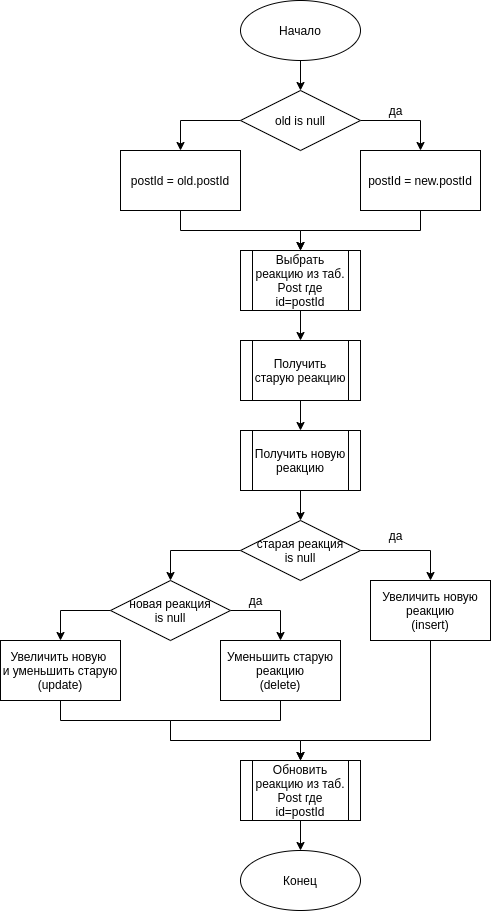
\includegraphics[width=0.8\linewidth]{img/trigger_change_reaction}

\lstinputlisting[language=SQL,linerange={0-16},caption=получить ленту (идентификаторы записи) ]{code/db.sql}
\lstinputlisting[language=SQL,linerange={18-29},caption=получить краткую информацию (json) о друзьях]{code/db.sql}
\lstinputlisting[language=SQL,linerange={31-42},caption=получить идентификаторы всех общих друзей]{code/db.sql}
\pagebreak
\lstinputlisting[language=SQL,linerange={44-82},caption=искать людей по имени]{code/db.sql}

\lstinputlisting[language=SQL,linerange={85-120},caption=Триггер изменении статистику реакций записи]{code/db.sql}
\lstinputlisting[language=SQL,linerange={123-150},caption=Триггер проверки правильности имени]{code/db.sql}

\vbox{}

\section*{Вывод}

В этом разделе было выполнен проектирование базы данных.
В функциях и триггерах я использовал такие функции Postgresql, как массив и json, это просто для того, чтобы практиковать знания, полученные в курсе по базам данных.
Поскольку база данных является наиболее сложным для масштабирования компонентом системы, на уровне базы данных будут выполняться только действительно необходимые функции.